\documentclass{standalone}

\usepackage[dvipsnames]{xcolor}
\usepackage{tikz}

\begin{document}

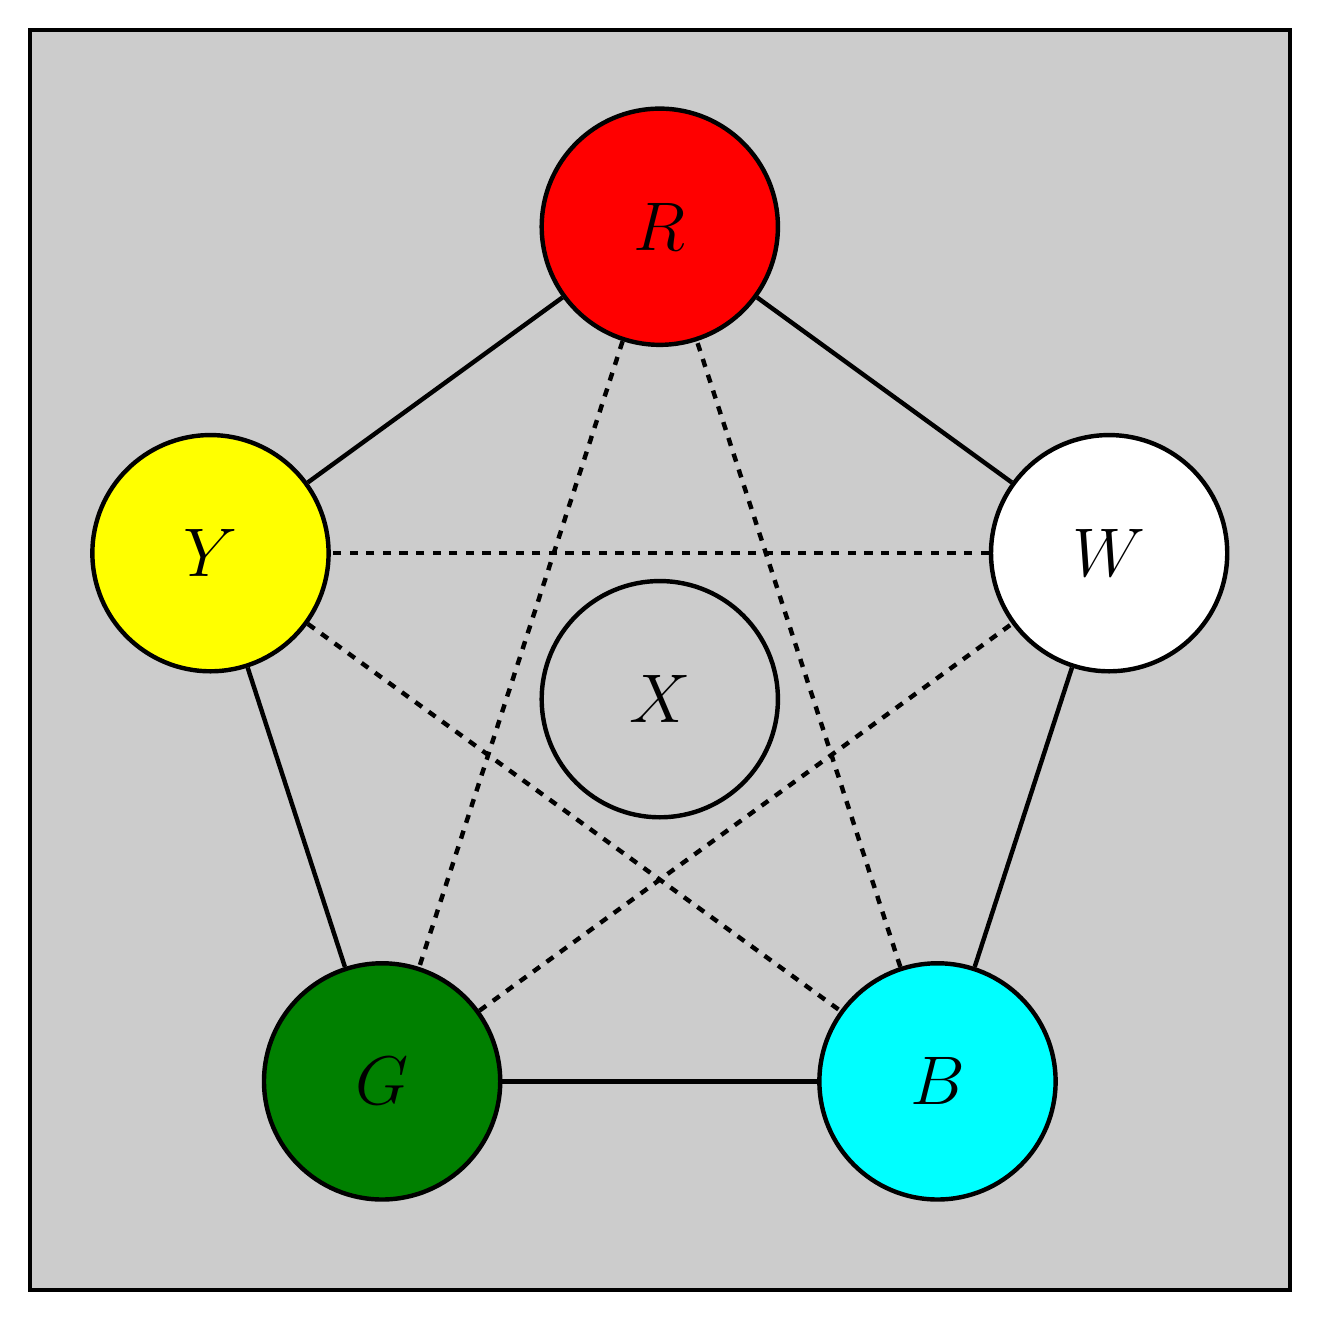
\begin{tikzpicture}
  \draw[ultra thick, fill=gray!40] (-8,-7.5) -- (-8,8.5) -- (8,8.5) -- (8,-7.5) -- cycle;

  \node[draw, circle, minimum size=3cm, fill=Red, ultra thick] (r) at (90:6) {\Huge{$R$}};
  \node[draw, circle, minimum size=3cm, fill=Yellow, ultra thick] (y) at (162:6) {\Huge{$Y$}};
  \node[draw, circle, minimum size=3cm, fill=Green, ultra thick] (g) at (234:6) {\Huge{$G$}};
  \node[draw, circle, minimum size=3cm, fill=Cyan, ultra thick] (b) at (306:6) {\Huge{$B$}};
  \node[draw, circle, minimum size=3cm, fill=White, ultra thick] (w) at (18:6) {\Huge{$W$}};
  \node[draw, circle, minimum size=3cm, ultra thick] (x) at (0,0) {\Huge{$X$}};

  \draw[ultra thick] (r) -- (y);
  \draw[ultra thick] (y) -- (g);
  \draw[ultra thick] (g) -- (b);
  \draw[ultra thick] (b) -- (w);
  \draw[ultra thick] (w) -- (r);
  \draw[ultra thick, dashed] (r) -- (g);
  \draw[ultra thick, dashed] (g) -- (w);
  \draw[ultra thick, dashed] (w) -- (y);
  \draw[ultra thick, dashed] (y) -- (b);
  \draw[ultra thick, dashed] (b) -- (r);
\end{tikzpicture}

\end{document}
